% !TEX root = presentation.tex
\begin{frame}
	\frametitle{conclusion}
	\todo[inline]{Conclusion?}
    \note{\textbf{[Name]} Conclusion?}
\end{frame}

\plain{	
    \begin{center}
    	\LARGE{questions?}
    \end{center}		
	\begin{columns}
		\begin{column}[b]{.5\textwidth}
			\begin{center}
				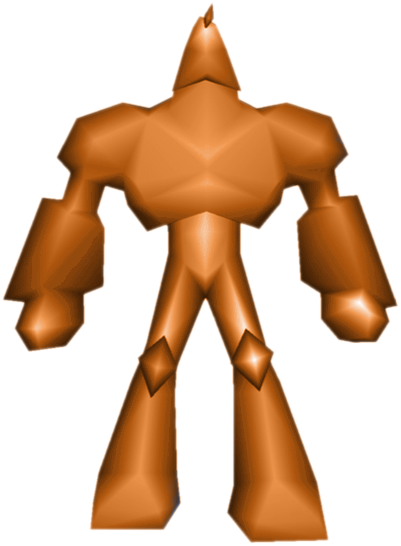
\includegraphics[
					width=\textwidth, 
					height=0.7\textheight,
					keepaspectratio=true
				]{./img/4_conclusion/finalresultNoPN.png}

				\small{triangles}
			\end{center}
		\end{column}
		\begin{column}[b]{.5\textwidth}
			\begin{center}
				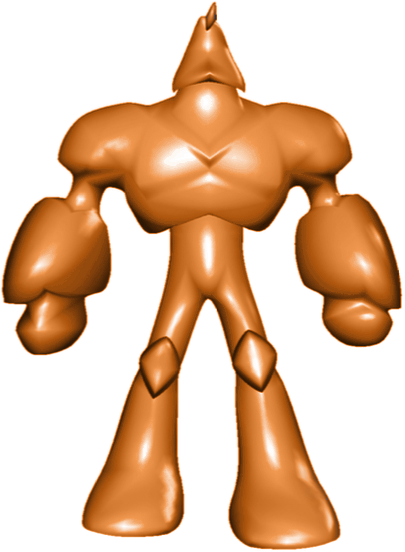
\includegraphics[
					width=\textwidth, 
					height=0.7\textheight,
					keepaspectratio=true
				]{./img/4_conclusion/finalResultPN.png}								

				\small{pn triangles}
			\end{center}
		\end{column}
	\end{columns}
}